% ================= EXPERIMENTS =================
\section{Experiments}
\label{sec:experiments}

\subsection{O1: restoration with a known kernel}
\label{sec:truepsf}
Before estimating anything, the non-blind step was checked with the \emph{true} PSF on the
development sources (1{,}440 trials over lengths, angles and noise levels; Fig.~\ref{fig:truepsf}).

\begin{figure}[h]
\centering
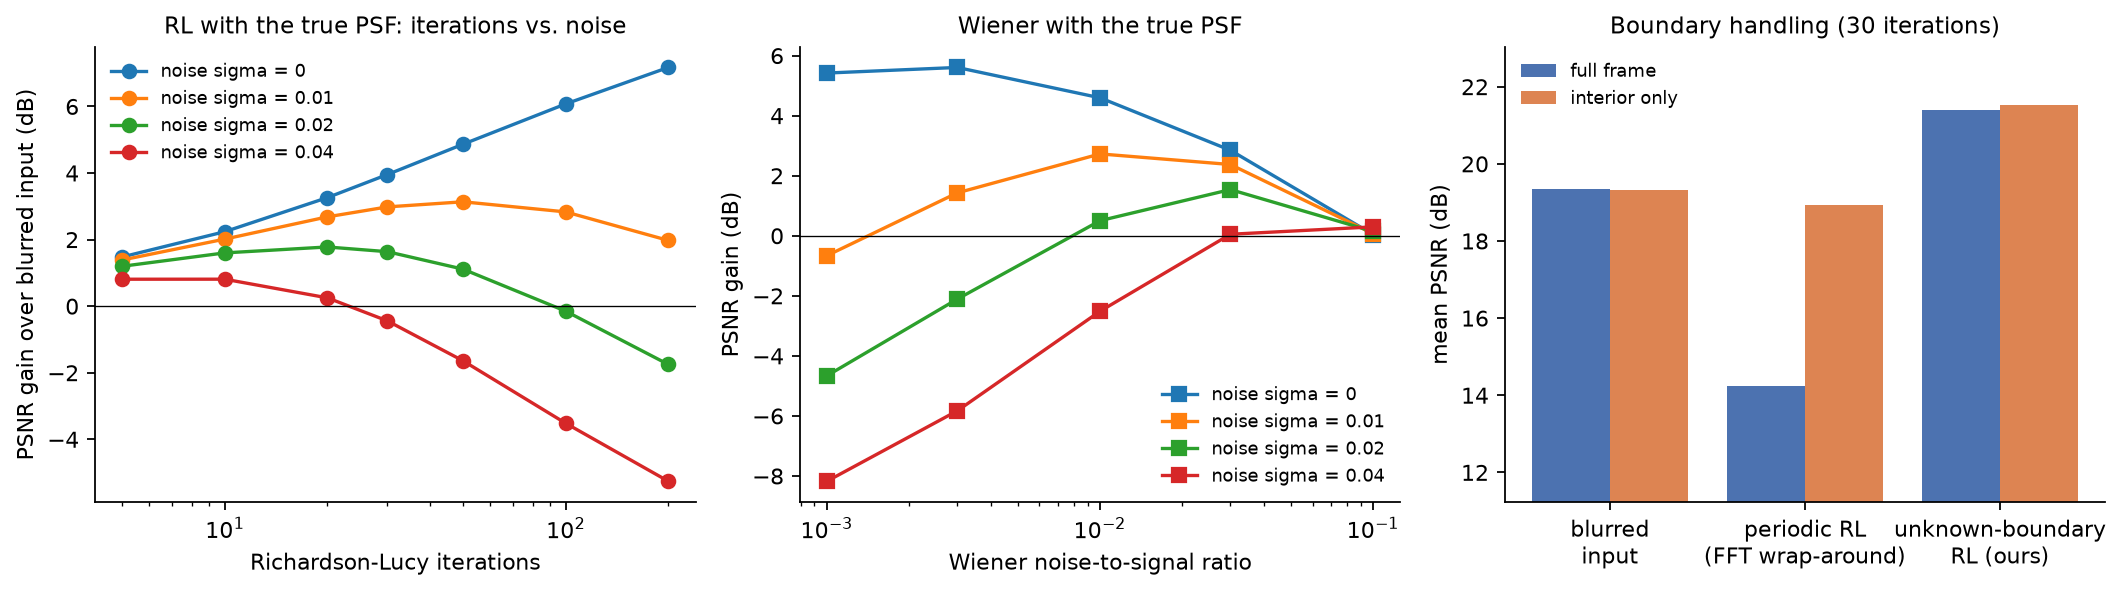
\includegraphics[width=\textwidth]{01_true_psf.png}
\caption{Restoration with the true PSF. Left: RL gain vs.\ iterations for four noise levels.
Middle: Wiener gain vs.\ noise-to-signal ratio. Right: boundary handling at 30 RL iterations.}
\label{fig:truepsf}
\end{figure}

\begin{itemize}
  \item \textbf{RL iterations depend on noise.} Without noise the gain keeps growing (+7.2\,dB at
        200 iterations); at $\sigma=0.04$ it peaks at about 10 iterations and becomes negative
        beyond 20, because RL then fits the noise. Stopping by the discrepancy principle (residual
        reaches the estimated noise level, $\tau=1$) gives a positive gain at every noise level:
        $+4.8$, $+2.3$, $+1.5$ and $+0.7$\,dB at $\sigma = 0, 0.01, 0.02, 0.04$. All synthetic
        restorations use this rule.
  \item \textbf{Boundaries matter.} Periodic RL wraps the image around, and the ringing this
        causes at the borders drops full-frame PSNR from 19.4\,dB (blurred) to 14.2\,dB.
        Unknown-boundary RL reaches 21.4\,dB on the full frame and 21.5\,dB in the interior.
  \item \textbf{Wiener} needs its noise-to-signal ratio matched to the noise level (best NSR
        moves from $0.003$ to $0.1$ as $\sigma$ grows); a mismatched NSR loses up to 8\,dB.
\end{itemize}
